\documentclass[]{article}

\usepackage{fullpage}
\usepackage{xcolor}
\usepackage{amsmath}
\usepackage{tikz}
\usetikzlibrary{automata,positioning,arrows.meta}

\usepackage{enumitem}
\usepackage{cleveref}
\crefname{enumi}{problem}{problems}

% Level
\newcommand{\Level}[1]{{\color{blue} $\langle$#1$\rangle$}}

\title{Sample Problems}
\author{Easy Theory}
\date{Last Updated: \today}

\begin{document}

\maketitle

\section*{How to Use these Problems}

This is a core dump of problems to practice in theory of computation.
This should give you a good idea of the types of questions that we will ask on an exam.
This list intentionally includes a few questions that are too long or difficult for exam conditions.
The list of questions is divided up into 5 difficulties: \Level{1} through \Level{5}, where \Level{3} is the maximum difficulty that we would expect on an exam. They are interpreted to mean as follows:
\begin{itemize}
	\item \Level{1}: should be able to solve within 5 minutes.
	\item \Level{2}: should be able to solve in 10-15 minutes (or at least see the approach that quickly).
	\item \Level{3}: should be able to solve within 30 minutes (or at least see the approach that quickly).
	\item \Level{4}: a very hard homework problem, likely taking a few hours.
	\item \Level{5}: either an open problem, or requires many hours of deep thought.
\end{itemize}

Try to not solve every single one of these problems. 
Instead, try to pick a \textit{sample} set of problems that you think would be most beneficial.
For instance, it would be a terrible idea to only work on \Level{1} problems, or only on \Level{5} problems. 

Discussing solutions to these problems is very beneficial, but \textit{only if} you have made an honest attempt at solving them yourself.
If you're getting stuck on a particular problem, try to understand \textbf{why} you are getting stuck on those problems, and try to remedy where the approaches are not clear.
If you're missing points consistently on coursework, try to come back to these problems to see why you are missing them.

\framebox[\textwidth]{Don't aim for ``understanding'' or ``regurgitating'' the solutions; instead aim for \textbf{\textit{mastery}}.}

\pagebreak

\tableofcontents

\pagebreak

\begin{enumerate}

\section{DFAs}

\item Produce a state diagram of a DFA for the following languages:
\begin{enumerate}

\item \Level{1} All strings except $\varepsilon$.

\item \Level{1} The language $\{\varepsilon, a, ab\}$.

\item \Level{1} All strings of length at most 3.

\item \Level{1} All strings that end in 010.

\item \label{ex2017prod1} \Level{1} All strings having at least one 0.

\item \label{ex2017fprod1} \Level{1} All strings starting with a 0.

\item \label{ex2017prod2} \Level{2} All strings such that their binary representation is not divisible by 3.

\item \Level{2} All strings except 010.

\item \Level{2} All strings that have the same number of 01 substrings as 10 substrings.

\item \Level{2} All strings that contain 0100 as a substring.

\item \Level{2} All strings that have 011 as a substring at least twice.

\item \Level{2} All strings over $\Sigma = \{0\}$ that have the same number of 0 and 00 substrings (Hint: what strings are actually in the language?)

\item \label{ex2017fprod2} \Level{3}  All strings that do not contain the subsequence 010.

\item \Level{3} All strings that do not contain the subsequence 010.

\end{enumerate}

\item \Level{2} For a language $L \subseteq \{0,1\}^\star$, let $L^c = \{w^c : w \in L\}$, where $w^c$ means that every 0 in $w$ is a 1 in $w^c$, and every 1 in $w$ is a 0 in $w^c$.
Prove that if $L$ is a regular language, then $L^c$ is a regular language.

\item \Level{2} Give a formal description of a DFA (by identifying all 5 parts precisely) that recognizes $L = \{w \in \{0,1\}^\star :$ the number of 1's in $w$ is a multiple of 355\}.

\item  \label{ex2017fsquaredouble} \Level{2} Let $Square(L) = \{ ww : w \in L\}$, and $Double(L) = \{wx : w, x \in L \}$.
Explain why, in general, $Square(L) \ne Double(L)$.

\item \Level{2} I am running for office and my three aides have each designed a DFA to solve a problem we are having in gathering voters (indeed each DFA describes, in some format, the voters we want to target).
However, all three are having trouble coordinating since they have each designed their DFAs differently, but also that their DFAs do not have the same language.
Since the election is coming soon, we cannot possibly target all voters in the languages in at least one of the DFAs.
And we cannot target just the voters that are in common with the three DFAs, because we project I won't win the election then.
We decide to target the voters that are in a \textit{majority} of the given DFAs.

Suppose the three DFAs are $D_1, D_2, D_3$, written as $D_i = (Q_i, \Sigma, \delta_i, q_{0,i}, F_i)$ for $i \in \{1,2,3\}$.
Design a DFA $D$ that accepts the following language:
\[
L = \{ w \in \Sigma^\star : w\;\text{is in at least two of $L(D_1), L(D_2), L(D_3)$}\},
\]
based on $D_1, D_2, D_3$.
Specify all 5 pieces of $D$ in terms of those of $D_1, D_2, D_3$.
Argue why your construction works.

\item \Level{2} True or false: if one repeatedly deletes states from $M$ that have no incoming transitions from other states, and proceeds until there are no such states to obtain a DFA $M'$, then $L(M) = L(M')$.

\item \Level{2} True or false: if $\Sigma=\{0,1\}$, produce DFA $M'$ by changing every 0 transition in $M$ to a 1 transition in $M'$, and vice versa. Then $L(M) \cap L(M') = \emptyset$.

\item \Level{2} Let $M$ be a DFA, and consider applying closure under complement to get a DFA for $\overline{L(M)}$; call it $M'$. 
Show that if $M$ has the smallest number of states possible for any DFA to recognize $L(M)$, then $M'$ has the same for $\overline{L(M)}$.

\item \Level{3} For a string $z$, let $|z|_x$ be the number of occurrences of $x$ in $z$.
For example, {\tt |banana|}$_{\tt ana} = 2$. 
Now consider each of the following languages; you can assume without proof that they are regular.
Determine whether or not they are finite languages, and explain.
\begin{enumerate}
	\item $\{z \in \{0,1\}^\star : |z|_0 = |z|_{00} = |z|_{1} = |z|_{11}\}$.
	\item $\{z \in \{0,1\}^\star : |z|_{00} = |z|_{11} = |z|_{000} = |z|_{111}\}$.
	\item $\{z \in \{0,1\}^\star : |z|_0 = |z|_{1} = |z|_{01} = |z|_{10}\}$.
\end{enumerate}

\item \Level{3} Let $\Sigma_{2} = \{0, 1\}$, and define $\Sigma = \Sigma_{2}^3$. Informally, $\Sigma$ is the set of triples of the form $(a, b, c)$ where $a, b, c$ are single binary digits. Consider a string $s \in \Sigma^\star$: it is a sequence of such triples. We want to ``verify" binary addition of numbers in the first two coordinates by checking that it is equal to the third. Let $A$ be the language of such triples such that the concatenation of the first coordinates, as a number, and the concatenation of the second coordinates, as a number, sum to be equal to the third. For example, if $w = (0, 1, 1)(1,1,1)(0,0,1)(1,0,1)$, this is encoding $0101_2 + 1100_2 = 1111_2$, which is false; therefore, $w \notin A$. Prove that $A$ is regular.

\item \Level{3} After observing your DFA construction skills, a group called the {\tt SuperSecretDFA} organization has hired you. This group markets on its website that ``Our single DFA is the smallest and most efficient of any regular language over $\{0,1\}$.''
By this, they mean that if you present their black box program with a regular language $L$, then it will produce a DFA with the smallest number of states that recognizes $L$.

We do not know the exact details of their black box, but they have generously noted that a DFA is the underlying object.
Most likely, the machine produces a copy of their DFA $D$, adjusts $D$'s transition function, and deletes all unnecessary states (or runs some DFA minimization algorithm) to give you the ``optimized'' DFA $D'$.

Because you were so considerate when interviewing the group, they also divulged to you that their DFA $D$, before copying, has a fixed number of states $n$, and at no point do they increase the number of states beyond $n$ (for generation efficiency reasons).

After hearing this information, you become skeptical of their machine's capability.

Describe a regular language $L$ that their super secret DFA cannot possibly recognize only knowing the number of states ($n$) it has, and give a convincing argument as to why it cannot recognize $L$.

\item \label{dfa_equal_no_product} \Level{4} Devise an algorithm that, on input two DFAs $D_1, D_2$, outputs True if $L(D_1) = L(D_2)$, and false otherwise.
However, you may not use any techniques other than the definition of a DFA, and any tools from prerequisite material (i.e., you may not use the product construction or other closure properties here).

\subsection{Product Construction}

For these problems, just formally \textit{describe} a DFA that recognizes $L$; don't attempt to draw the DFA as it may be too large. 
Instead, all you need to specify is a formal description of the 5 pieces of a DFA; $Q, \Sigma, \delta, q_0$, and $F$.

\item Produce a DFA for the following languages:
\begin{enumerate}


\item \Level{1} The intersection of the languages in \cref{ex2017prod1,ex2017prod2}.

\item \Level{2} The symmetric difference of the languages in \cref{ex2017prod1,ex2017prod2}.

\item \Level{2} All strings such that the number of 0s is even, the number of 1s is divisible by 3, and the length of the string is divisible by 5.

\item \Level{2} The intersection of the languages (and complementing the second) of \cref{ex2017fprod1,ex2017fprod2}.

\item \Level{2} Consider the following languages:
\begin{itemize}
	\item $L_1 = \{ w \in \{0,1,2\}^\star : w$ either starts with a 0 and ends with a 0, or starts with a 1 and ends with a 1, or is $\varepsilon\}$,
	\item $L_2 = \{w \in \{0,1,2\}^\star : w$ starts with 1$\}$, and
	\item $L_3 = \{w \in \{0,1,2\}^\star : w$ is the ternary representation of an integer multiple of 4$\}$.
\end{itemize}
Construct a DFA that recognizes the language $L_2 \cap (L_1 \cup \overline{L_3})$.
\end{enumerate}



\item \Level{2} Suppose two DFAs $D_1, D_2$ have $n_1, n_2$ states each, and $f_1, f_2$ final states each. Now form the DFA $D$ from the product construction for the \emph{union} of their languages. How many final states does $D$ have?

\item \Level{2} Related to \cref{dfa_equal_no_product}, devise an algorithm that, on input two DFAs $D_1, D_2$, outputs True if $L(D_1) = L(D_2)$, and false otherwise (here you \textit{can} use the product construction).

\subsection{NFAs}

\item \label{ex2017fnfa} \Level{1} Consider the following NFA:

\begin{center}
	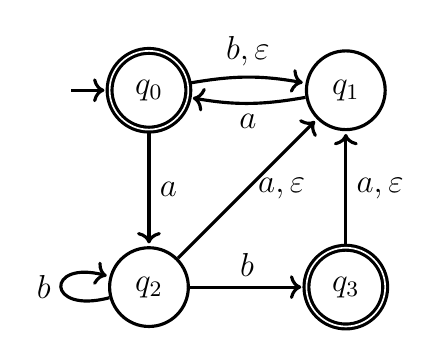
\begin{tikzpicture}[shorten >=1pt,node distance=2.5cm,on grid,auto,initial text={},font=\large,every state/.style={align=center,minimum size=1cm},line width=0.4mm] 
	\node[state,accepting,initial,inner sep=5pt] (q_0)   {$q_0$}; 
	\node[state] (q_1) [right=of q_0] {$q_1$}; 
	\node[state] (q_2) [below=of q_0] {$q_2$}; 
	\node[state,accepting] (q_3) [right=of q_2] {$q_3$};
	\path[->] 
	(q_0) edge [bend left=10] node {$b, \varepsilon$} (q_1)
	edge node {$a$} (q_2)
	(q_1) edge [bend left=10] node {$a$} (q_0)
	(q_2) edge [right] node {$a, \varepsilon$} (q_1)
	edge [loop left] node {$b$} ()
	(q_2) edge node {$b$} (q_3)
	(q_3) edge [right] node {$a, \varepsilon$} (q_1);
	\end{tikzpicture}
\end{center}

Convert this NFA into an equivalent DFA.

\item \Level{1} Show that if $L$ is regular, then $OIF(L) = \{1w : w \in L \}$ is also regular.

\item \Level{2} Show that if $L$ is regular, then $\#(L) = \{1^{|w|} : w \in L\}$ is also regular.

\item \Level{2} Show that if $L$ is regular, then $L^{rev} = \{w^{rev} : w \in L\}$ where $w^{rev}$ is the reverse of $w$, is also regular (Hint: be careful.)

\item \Level{3} Show that if $L$ is regular (and the alphabet contains 1, but is not necessarily equal to 1), then $\#^{-1}(L) = \{w : 1^{|w|} \in L\}$ is also regular.



\subsection{Regular Expressions}

\item \Level{1} Convert the DFA for \cref{ex2017fprod1} into an equivalent regex.

\subsection{Pumping Lemma for Regular Languages}

\item \Level{2} Recall the definition of $Square(L)$ from \cref{ex2017fsquaredouble}. 
Show that there is a regular language $L$ for which $Square(L)$ is not regular.

\item \Level{4} Let $L$ be any unary language, regular or not. Show that $L^\star$ is regular.

\subsection{Regular Grammars}

\item \Level{1} Convert the NFA from \cref{ex2017fnfa} into an equivalent regular grammar.

\section{Context-Free Languages}

\subsection{CFGs}

\item \label{summer_2017_cfg} \Level{1} Produce a CFG $G$ for $L_1 \cup L_2$ where $L_1 = \{0^n 1^n 2^m 3^m : n,m \ge 0 \}$ and $L_2 = \{0^n 1^m 2^m 3^n : n, m \ge 0 \}$.

\item \Level{1} Recall the definition of $Double(L)$ from \cref{ex2017fsquaredouble}. Show that if $L$ is a CFL, then $Double(L)$ is also a CFL.

\item \Level{2} Give an example of a context-free language $L$ that, for \textit{any} CFG with language $L$, requires \textit{at least} 2 variables. 
Prove that there is no CFG for $L$ with only 1 variable.\footnote{Unfortunately the problem of determining if a given CFG is minimal with respect to the number of variables is undecidable, so brute-force may or may not work here.}

\item \Level{4} Consider the string $a^n$ for some integer $n$. The language $\{a^n\}$ clearly is regular (it has only 1 string), and hence is context-free. A simple CFG for it is $S \to a\cdots a$. 

We will consider the \textit{complexity of $a^n$} to be the following: we sum for every rule the number of variables and terminals in that rule as well as the $\to$ symbol. For example, the complexity of $a^n$ is at most $n+2$ since the grammar above has 1 variable, $n$ occurrences of the symbol $a$, and one $\to$ symbol.

We can improve this in some cases. For $a^9$, we can make the grammar $S \to BBB, B \to aaa$, which has 5 variable occurrences, 2 $\to$ occurrences, and 3 terminals, which sums to 10 (better than the trivial bound of 11).

For what $n$ can we have a better complexity than $n+2$, and what $n$ require $n+2$?
Write a program to generate the complexity (with a CFG with that complexity) for all $n \le 100$. 
Discuss how you designed your program, as well as discuss what you believe the ``correct'' answer is. 
Can you say much about complexities for much larger $n$ (say, at least $10^5$)?

\subsection{CNF}

\item \Level{2} Convert the CFG in \cref{ex2017fcfg} into CNF.

\item \Level{2} Consider any regular grammar. If we wanted to convert it into CNF, show that one of the five steps in the conversion process can be skipped.

\subsection{PDAs}

\item \label{ex2017fcfg} \Level{1}  Convert the following CFG into an equivalent PDA.
\begin{align*}
S &\to aBb\\
B &\to ac \;|\;S\;|\;\varepsilon
\end{align*}


\item \Level{1} Produce an equivalent PDA $P$ for the grammar in \cref{summer_2017_cfg}.

\item \Level{2} Prove or disprove the following statements:
\begin{enumerate}
	\item Stacks are getting expensive lately! I limit my PDAs to only have a maximum stack height of 50, and if during a computation the PDA tries to push on a stack with height of 50, the computation terminates. My model of PDAs then still recognizes the context-free languages.
	\item The energy it is taking for PDAs to take a transition where it reads off of the input is increasing, so it may be a good idea to allow ``breaks" between them. I want every accepting computation of every string to consist of at least 1 $\varepsilon$-transition between each character read from the input, without worrying about what happens to the stack. Call these machines $\varepsilon$-PDAs. Then $\varepsilon$-PDAs still recognize the context-free languages.
\end{enumerate}

\item \Level{3} Consider two strings $w = w_1 \cdots w_n$ and $x = x_1 \cdots x_m$. We want to consider \textit{edits}: insertions, deletions, and substitutions. All such edits are equal; they have a ``cost'' of 1.

The \emph{edit distance of $w, x$}, denoted ${\textsf{ED}}(w,x)$, is the minimum size of a sequence of edits over all possible sequences of edits on $w$ to have $w$ equal to $x$. For example, if $w = abb$ and $x = bc$, then the (minimum) edit distance is 2; one such edit sequence is deleting $a$, and substituting the second $b$ for a $c$. Also, there is no edit sequence of length 1 to transform $abb$ into $bc$.

Consider the following language for a given value of $k$ (where $x^{rev}$ is the reverse of string $x$):
\[
\textsf{Edit(k)} = \{ w \# x^{rev} : w, x \in \{a, b, c\}^\star, \textsf{ED}(w,x) \le k  \}.
\]
In other words, this language has all strings of the form $w\# x^{rev}$ where the edit distance is less than $k$.
\begin{enumerate}
	\item Produce a PDA $P$ that recognizes $\textsf{Edit(1)}$.
	\item Convert $P$ into an equivalent CFG $G$ using the techniques from class (Hint: write a program to output all the rules.)
	\item Show that for any fixed value of $k$ that $\textsf{Edit}(k)$ is context-free. (Hint: generalize $\textsf{Edit}(1)$.)
\end{enumerate}

\item \Level{3} A \textit{recursive automaton} is a 3-tuple $(M, P, \{D_k : k \in M \})$, where $M$ is a finite set of \textit{module names}, $P \in M$ is the \textit{start module}, and for each $k \in M$, there is an NFA $D_k$ over the alphabet $\Sigma \cup M$, and have pairwise disjoint states. 

In other words, the recursive automaton is a collection of NFAs that can ``call'' other NFAs in $M$ via a transition, including themselves. 
The notion of computation from NFAs extends to here as well, except now we keep a \textit{stack} of which modules ``called'' which other modules, and in what order. 
We push onto this stack if we call another module, and we pop if we end in a final state of that module (and return to the module then on the top of the stack).
We accept a string iff the string is in a final state of $P$ (the start module) and the stack of module calls is empty.
		
Prove that the languages of recursive automata are exactly the CFLs.

\subsection{Pumping Lemma for Context-Free Languages}

\item \Level{2} For a language $L$, let $\textsf{Shuffle}(L)$ be the following language:
\[
\{ w : x \in L, |w| = |x|,\;\text{and $w$ is a permutation of the letters in $x$} \}.
\]
\begin{enumerate}
	\item Prove that regular languages are \emph{not} closed under shuffle. (Hint: use part (b))
	\item Prove that context-free languages are \emph{not} closed under shuffle.
\end{enumerate}

\item \Level{2} Let $L = \{w \in \{0, 1\}^\star : |w|\;\text{is a power of $n$, and $n$ is even}\}$. Prove that $L$ is not context-free.

\item \Level{2} Recall the definition of $Square(L)$ from \cref{ex2017fsquaredouble}. 
	Show that there is a CFL $L$ for which $Square(L)$ is not a CFL.

\item \Level{2} Produce two non-context-free languages $L_1, L_2$ such that $L_1 \cap L_2$ is context-free.

\item \Level{3} Produce a non-context-free language $L$ such that $L^\star$ is context-free.

\item \Level{4} Produce a non-context-free language $L$ such that $\overline{L}$ is also non-context-free.

\item \Level{4} Produce two non-context-free languages $L_1, L_2$ such that $L_1 L_2$ is context-free.

\item \Level{4} Show that any unary context-free language is regular.

\section{Turing Machines}

\item \Level{2} Write a low-level description of a TM to recognize the language:
\[
\{w \in \{0, 1\}^\star : \#_0(w) = (\#_1(w))^2 \}.
\]

\item \Level{2} A \textit{backtracking Turing Machine} (BTM) is just like a normal TM except that there is another transition that ``backtracks''--when taken from state $q$, this transition instantly resets the tape contents and tape head location to be exactly when the machine was last in state $q$. If the machine was not in state $q$ before, the tape does not change.

Prove that the languages recognized by BTMs are equivalent to those recognized by ``standard'' (deterministic, single-tape) TMs.

\item \Level{2} A \textit{stack Turing machine} (STM) is like a normal TM except in every tape cell there is, in addition to a symbol, a stack. On each transition taken, the machine, in addition to modifying the cell's symbol and move left or right, can push or pop from that individual cell's stack (or both, or neither, as how a PDA can). If the STM attempts to pop from a cell's stack that is empty, the computation terminates.

Prove that the languages recognized by STMs are equivalent to those recognized by ``standard'' (deterministic, single-tape) TMs.

\section{Decidability}

\item \Level{2} Let $L$ be the language:
\begin{align*}
\{ \langle D, N, R, G, P \rangle :\;\text{$D$ is a DFA, $N$ is an NFA, $R$ is a regex, $G$ is a regular grammar,}\\
\text{$P$ is a PDA, and $L(P) \subseteq ((L(D) \cap L(N)) \cup \overline{L(R)}) L(G)$ }   \}
\end{align*}
Show that $L$ is decidable (Hint: what is the intersection of a CFL and a regular language?)

\item \Level{2} Let $WEIRD_{NFA} = \{ \langle M \rangle : M$ is an NFA, $M$ has at most 7 states, accepts $\varepsilon$, and $L(M)$ is infinite$\}$.
Show that $WEIRD_{NFA}$ is decidable.

\item \Level{2} Let $L$ be a language, and let $\textsf{Power}(L)$ be:
\[
\{ w^n : w \in L, n \ge 0 \}.
\]
Prove that if $L$ is recognizable, then $\textsf{Power}(L)$ is also recognizable.

\item \Level{3} I'm concerned that the NFAs we usually deal with are ``too large'' and that we can make them even simpler. I want to determine, given an NFA $N$, whether or not there is some other NFA with fewer states than that also recognizes the language $L(N)$. 

However, this may not be ``minimal'' enough, because there could be still another NFA with fewer transitions than $N$ still with the same number of states and language $L(N)$. 

Formally state this problem. Then show that this problem is decidable.

\item \label{regex_crossword} \Level{3} You are given a grid $A[1..m][1..n]$ ($m$ rows, $n$ columns) as well as $m$ regular expressions $R_1, \cdots, R_m$ corresponding to each row, and $n$ more regular expressions $C_1, \cdots, C_n$ corresponding to each column. The alphabet of all regexes is $\Sigma$. Your task is to determine if there is a way of assigning a character in $\Sigma$ in each of the cells of $A$ such that the concatenation of the cells in row 1 (from left to right) is a string in $L(R_1)$, row 2's concatenation is a string in $L(R_2)$, as well as for all the other row and column regexes (columns concatenate from top to bottom). We say that this input has a \textit{solution} if there is such an assignment. 

For example, here is a graphical representation of a possible input with $\Sigma = \{a, b\}$:

\begin{table}[!htb]
	\centering
	\begin{tabular}{llll}
		\cline{2-4}
		\multicolumn{1}{l|}{$(bba)^\star$} & \multicolumn{1}{l|}{} & \multicolumn{1}{l|}{} & \multicolumn{1}{l|}{} \\ \cline{2-4} 
		\multicolumn{1}{l|}{$b(a^\star b)^\star$} & \multicolumn{1}{l|}{} & \multicolumn{1}{l|}{} & \multicolumn{1}{l|}{} \\ \cline{2-4} 
		&     $(a \cup bb)^\star$                 &       $(ba)^\star ab$                &   $((ba)^\star \cup (ab)^\star)^\star$                
	\end{tabular}
\end{table}

Let the language $\textsf{RegexCrossword}$ be the set of all instances $\langle A, R_1, \cdots, R_m, C_1, \cdots, C_n\rangle$ where $A$ is an $m \times n$ grid, $R_1, \cdots, R_m, C_1, \cdots, C_n$ are regexes, and there is a solution to $A$ as described above. Show that $\textsf{RegexCrossword}$ is decidable. (Hint: brute-force.)

\item \Level{4} Let $\textsf{RegexCrosswordWord}$ be the language similar to that in \cref{regex_crossword}, except now the cells can be filled with a string in $\Sigma^\star$ instead of just a single character. Is $\textsf{RegexCrosswordWord}$ decidable? Recognizable? 

\section{Undecidability}

\item \Level{2} I want to know if my compiler, represented as a CFG, conforms to a given specification, also represented as a CFG. Let $L = \{\langle G_1, G_2 \rangle : G_1, G_2$ are CFGs and $L(G_1) \subseteq L(G_2)\}$. Prove that $L$ is undecidable.

\item \Level{2} Prove that $SUPEROBEY_{TM} = \{ \langle M_1, M_2 \rangle : M_1, M_2$ are TMs, $L(M_1) \subseteq L(M_2)$, and $L(M_2)$ contains at least 1 more string than $L(M_1)$ does$\}$ is not decidable. (Hint: $\mathsf{E}_{\mathsf{TM}}$)

\item \Level{2} Prove that $INTERCFL_{TM} = \{ \langle M \rangle : M$ is a TM and $L(M)$ is the intersection of 2 CFLs, and $L(M)$ is also a CFL$\}$ is not decidable.

\item \Level{3} Let $M$ be a TM. Call $M$ a \textit{narcissistic} TM if $L(M) = \{ \langle M \rangle \}$; in other words, the only string that $M$ recognizes is its own description. We will assume, without proof, a theorem called the ``recursion theorem'' (see Sipser Chapter 6 if you're interested): \textit{any} TM has the ability, as its first step, to get its own description as a string.
\begin{enumerate}
	\item Show that a narcissistic TM exists.
	\item Let $L = \{ \langle M \rangle : M$ is a narcissistic TM$\}$. Prove that $L$ is not recognizable, and that $\overline{L}$ is not recognizable (Hint: reduce from a known non-recognizable language). 
\end{enumerate}

\item \Level{3} I am concerned that my Python program is too complicated, and can be simplified without changing its behavior. It would be nice if I can check whether there is such a simpler program. We aren't concerned with what ``simplified'' means other than the size of the program. Let $L = \{ \langle P \rangle : P$ is a Python program and there is no other Python program smaller in size than $|\langle P \rangle|$ with language $L(P)\}$. Show that $L$ is not recognizable (Hint: you may assume the recursion theorem of the last problem).

\end{enumerate}

\end{document}
